\documentclass[tikz, border=20pt]{standalone}

% Schriftart-Einstellungen gemäß Vorgabe
\usepackage{tgheros}
\renewcommand{\familydefault}{\sfdefault}

% TikZ-Bibliotheken
\usetikzlibrary{positioning, shapes, calc}

% Zentrale Stil-Definitionen
\tikzset{
    punkt/.style={
        circle,
        draw=black,          % Klare schwarze Kontur
        fill=white,          % Neutrale weiße Füllung
        minimum size=3.5mm,  % Definierte Größe für perfekte Kreise
        line width=0.7pt     % Professionelle Linienstärke
    }
}

\begin{document}
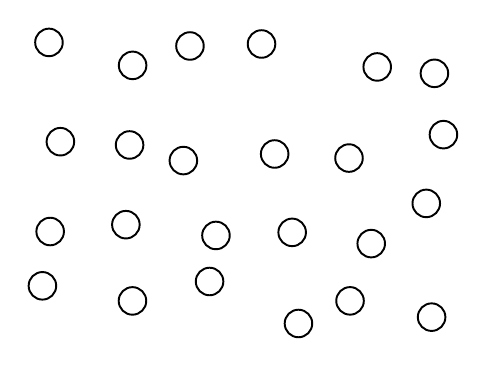
\begin{tikzpicture}

    % Um Überlappungen bei 24 Punkten sicher auszuschließen und dennoch 
    % eine unregelmäßige Optik zu erzielen, nutzen wir ein gestörtes Gitter.
    
    \pgfmathsetseed{150} % Fester Seed für reproduzierbare Verteilung

    \foreach \i in {0,...,23} {
        % Wir berechnen eine Gitterposition (6 Spalten x 4 Zeilen = 24 Punkte)
        \pgfmathsetmacro{\spalte}{mod(\i,6)}
        \pgfmathsetmacro{\zeile}{floor(\i/6)}
        
        % Basis-Abstand ist 1.0cm. Der maximale Zufalls-Offset (jitter) beträgt +/- 0.3cm.
        % Da der Durchmesser 0.35cm beträgt, ist eine Überlappung mathematisch ausgeschlossen.
        \node[punkt] at ({\spalte*1.0 + (rnd-0.5)*0.6}, {\zeile*1.0 + (rnd-0.5)*0.6}) {};
    }

\end{tikzpicture}
\end{document}